\chapter{Introduction} \label{chap:intro}

The purpose of this chapter is to introduce the motivation for the work, briefly describe the problem at hand and outline the work that will be developed, as well as the structure of the thesis.

\section{Motivation} \label{sec:motivation}

Collective software development requires the handling of merge conflicts, as conflicts between parallel work arise. Called merge conflicts, as they arise when this parallel work is merged, they vary in their difficulty of detection.
Common textual conflicts, where the same line is altered by multiple people, are automatically detected by version control systems, allowing amendments to be easily made. However not all conflicts are this easily detected and their introduction bring with it the addition of software bugs to the system. Semantic merge conflicts, in particular, are hard to detect, both by software and human review and remain a hard to solve situation. Given that around 30\% of developers do not even actively monitor for merge conflicts and of those who do, mostly do it with reactive strategies \citep{kn:lifecycle}, the ability to automatically detect these would be a great boon for the field of software development, especially as by developers own admissions, the longer a merge conflict is left unsolved, the harder it becomes to resolve it: “Untangling takes days instead of minutes when it gets too out of hand.” \citep{kn:lifecycle}.

The recent revolution in the field of Large Language Models (LLMs) may prove to add a valuable tool in tackling this.


\section{Problem} \label{sec:problem}

To manage the concurrent work of several developers in software projects, it is common to employ \emph{version control systems} (hereby referred as \emph{VCS}), which can be defined as "a system that manages the development of an evolving object. In other words, it is a system that records any changes made by the software developers." ~\citep{kn:vers_review}.

A significant task of version control is managing access to shared resources.
In the "classic scenario" a lock-modify-unlock paradigm was adopted, where a given file would be locked for modification while it is being modified, thus ensuring each resource can only be handled by one actor at a time. VCS's however, generally implement a copy-modify-merge mechanism: concurrent work can done on a resource, with joining the parallel work together handled by merges afterwards, with two "branches" of work merged into one ~\citep{kn:vers_ott}.

Merge conflicts arise when parallel work can't be clearly merged. Of this, several different types exist, as summarized by Tom Mens ~\citep{kn:tmens}:

Textual conflicts occur when the same textual elements of code are modified in both branches of a merge. For example, when the same line of code is modified by two people in their respective branches.

Syntactic conflicts arise from parallel changes that when merged don't generate textual conflicts, but the resulting merge creates code that is invalid given the languages rules. For example, programmer A renames a variable, while programmer B uses the variable somewhere (with the original name). There's no textual code, but the code won't compile due to the usage of an uninitialized variable.

Finally semantic conflicts occur when parallel changes don't trigger any conflict and are syntactically valid, but the resulting code doesn't behave as expected, or exhibits lost or new unexpected behaviour.

Most VCS's, such as Git, implement textual merge tools (ergo, they can only identify textual conflicts), however there are specialized tools that handle other types of merges: for example Turbomixer for syntactic merges~\citep{kn:tmens}. This focus on textual merging is generally fine as around 90\% of conflicts are textual ~\citep{kn:lcsd} and syntactic conflicts are easy to identify after merges, as errors will be clearly indicated and programs won't compile.
Semantic conflicts remain as both undetected by VCS's and hard to detect after merges. Thus, identifying methods to automatically identify and highlight semantic conflicts in merge commits has been a persistent problem and a source of study in this field~\citep{kn:nuno} ~\citep{kn:leuson} ~\citep{kn:leuson2}.


A motivating example of a merge conflict can be seen in a class "Cart", for a shopping app. Initially having just a method total\_cost that calculates the total cost given a percentage of discount, it is modified in branch A: a additional parameter for tax and the method is overloaded with another implementation that just calculates tax and not discount. Then, in branch B, a checkout method is added, which calls the original total\_cost method. After merging, no error appears, but the checkout function will be running the total\_cost tax method, expecting the calculation of a discount.

From here the conflict arises, as after merging the behaviour is altered: the checkout function which would calculate the cost with a discount, now instead uses the value given for discount to calculate tax. To identify this conflict, we would need to generate a test that would find evidence of this alteration: in this case finding that the checkout function is charging more money than expected.

\begin{figure}[t]
    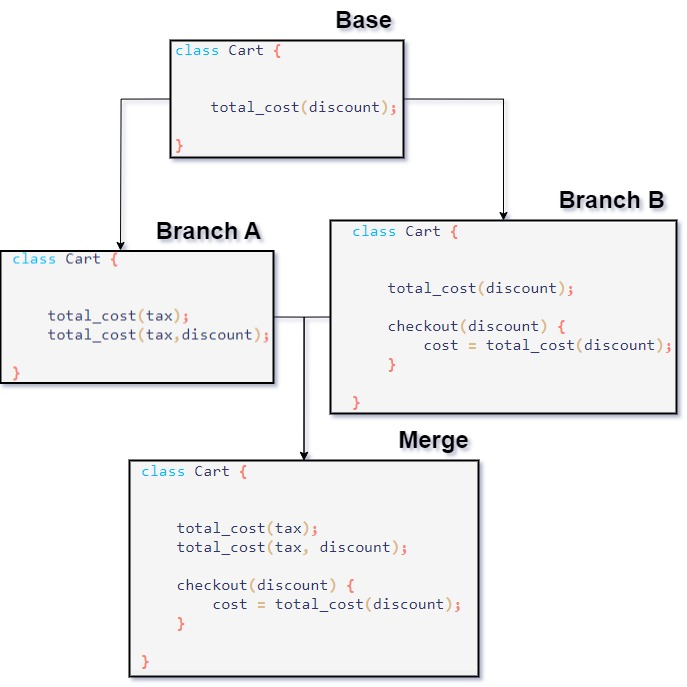
\includegraphics[width=0.86\textwidth]{conflict}
    \caption{Model of the presented conflict}
    \label{fig:arch}
\end{figure}

\section{Goal} \label{sec:goal}

The goal of the presented project is to develop an automated system that can detect possible merge conflicts in a merge and generate the necessary unit tests to identify it using a LLM, allowing for easier detection of this type of conflicts to be integrated into the version control workflow of developers.

\section{Approach} \label{sec:approach}

In previously developed work, a Domain-Specific Language was designed which describes the changes made in a three-way merge~\citep{kn:nuno}. This DSL provides a summarized report of a three-way merge. We will feed the DSL reports into ChatGPT and induce it to generate unit tests based on them which should help assess the presence of a semantic conflict originating from the merge.






\section{Thesis Structure} \label{sec:struct}


The first chapter introduces the topic and problem at hand.
The second chapter details existing related work on the topics at hand.
The third chapter introduces the proposed solution.
The fourth chapter gives a conclusion.